% aliveKat
\documentclass[aps,pra,superscriptaddress,reprint,nofootinbib]{revtex4-1}
% \documentclass[prb,reprint,nofootinbib]{revtex4-1} 
% \documentclass[pra,superscriptaddress,reprint,nofootinbib]{revtex4-1}
% \documentclass[prb,preprint,letterpaper,noeprint,longbibliography,nodoi,footinbib]{revtex4-1} 



% worry about formatting AFTER the text is written



\usepackage[utf8]{inputenc}
\usepackage{amsmath,amssymb,amsthm}
\usepackage{amsfonts}
\usepackage{graphicx}
\usepackage{float}
\usepackage{mathtools}
% \usepackage[usenames,dvipsnames]{xcolor}	
\usepackage{hyperref}
% \usepackage{siunitx}
\usepackage{textcomp}
\usepackage{subfiles}
\usepackage{comment}
% \usepackage[bottom]{footmisc}

\usepackage{silence}
\WarningFilter{revtex4-1}{Repair the float}

%\bibliographystyle{apsrev4-2}
%\setlength{\parindent}{0pt}

\newcommand{\abs}[1]{\left\lvert #1 \right\rvert}
\newcommand{\norm}[1]{\left\lVert #1 \right\rVert}
\newcommand{\ip}[2]{\langle #1,#2 \rangle}


\begin{document}
\title{Optical modelling of advanced gravitational wave detector configurations}

\author{James W. Gardner}
\email{u6069809@anu.edu.au}
\affiliation{%
College of Science, Australian National University, Acton, ACT, 2601, Australia 
}%

\author{Vaishali B. Adya}
% \email{vaishali.adya@anu.edu.au}
\affiliation{%
Centre for Gravitational Astrophysics, The Australian National University, Acton, A.C.T., 2601, Australia
}
\affiliation{%
OzGrav @ ANU, Australian Research Council Centre of Excellence for Gravitational Wave Discovery, Acton, A.C.T., 2601, Australia
}

\author{David McClelland}
% \email{david.mcclelland@anu.edu.au}
\affiliation{%
Centre for Gravitational Astrophysics, The Australian National University, Acton, A.C.T., 2601, Australia
}
\affiliation{%
OzGrav @ ANU, Australian Research Council Centre of Excellence for Gravitational Wave Discovery, Acton, A.C.T., 2601, Australia
}

\author{Daniel Töyra}
% \email{daniel.toyra@anu.edu.au}
\affiliation{%
Centre for Gravitational Astrophysics, The Australian National University, Acton, A.C.T., 2601, Australia
}
\affiliation{%
OzGrav @ ANU, Australian Research Council Centre of Excellence for Gravitational Wave Discovery, Acton, A.C.T., 2601, Australia
}

\date{\today}


%%%%%%%%%%%%%%%%%%%%%%%%%%%%%%%%%%%%%%%%%%
\begin{abstract}
% to-do todo
Abstract: ??? 

\end{abstract}

% {
% \let\clearpage\relax
\maketitle
% }
% \tableofcontents

%%%%%%%%%%%%%%%%%%%%%%%%%%%%%%%%%%%%%%%%%%
\section{Introduction}
\label{sec:introduction}

% gw’s and gw detectors
The first detection of gravitational waves in 2015 from the merger of two black holes~\cite{GW150914} opened a new frontier for astronomy. 
Gravitational waves are a prediction of the theory of General Relativity and represent ripples in the ``fabric of space-time'' that stretch and squish the lengths and durations between events. Gravitational wave detectors, such as the Advanced Laser Interferometer Gravitational-wave Observatory (aLIGO~\cite{AdvancedLIGO:2015}), are vast and complex experiments that rely fundamentally on the interference of light to detect minuscule changes in the lengths of the two long arms of an interferometer. Due to the mass scales required, detectable gravitational waves are only generated by the most massive of cosmic sources. With the initial generation of detectors having demonstrated that detection is possible, the natural question now is how to improve upon them to make detectors with higher sensitivity for all kinds of sources.


% motivate the need for optical modelling
Due to the complexity of the detectors, deriving analytic solutions for the expected signal and noise output due to a passing gravitational wave is difficult to do, especially exactly. %, and almost never into a closed form. 
While solutions are known for the current configurations, with each new proposed configuration a new set of non-trivial analytics needs to be done and as the proposals get more exotic the task only grows more difficult.
One solution to this is to look to optical modelling, numerical simulations of an optical system that can deliver fast results and let the researcher quickly ascertain the efficacy of a proposed configuration. 


% what we do
In this report, we demonstrate the use of an existing piece of optical modelling software, Finesse~\cite{finesse}, in a variety of gravitational wave detector configurations and compare against known analytics. In particular, we test the implementation of a non-linear element in Finesse in a simple cavity and then use the element to test proposed detector configurations with internal squeezing.


% report structure
This report is structured as follows.
In Section~\ref{sec:Finesse} we detail Finesse and what it does. In Sections~\ref{sec:basics}~\ref{sec:squeezing} we review the basics of interferometry and squeezing, respectively. In Section~\ref{sec:gwIFO} we detail the aLIGO configuration. In Section~\ref{sec:sqzcavity} we test the implementation of a non-linear element in Finesse against derived analytics. %, outside and inside of a cavity.
In Section~\ref{sec:aLIGOcomparison} we compare a model of the aLIGO configuration in Finesse to known analytics, with and without internal squeezing, for a variety of interferometer parameters.
We suggest areas for future work in Section~\ref{sec:future_work} and draw conclusions in Section~\ref{sec:conclusions}.


\section{Finesse} %- Optical modelling
\label{sec:Finesse}
% this section can be quite short

% what does finesse do, how does it do it
Finesse~\cite{finesse} (Frequency domain INterfErometer Simulation SoftwarE) is a piece of optical simulation software designed for modelling interferometer configurations. For a specified configuration of optical components, at each connecting node it calculates the light amplitudes for the carrier, the signal sidebands, and the quantum noise sidebands (see Sections~\ref{sec:basics}). By solving the appropriate matrix equations, it does all of this entirely in the frequency domain. By placing appropriate detectors at the output, Finesse is able to calculate the expected signal and quantum noise transfer functions and so the sensitivity of a proposed detector configuration (see Section~\ref{sec:gwIFO}).
Although not explored here, Finesse also is able to handle the spatial geometry of the configuration by modelling with Gaussian beams.


% what is new
Newly implemented in the development branch of Finesse is a non-linear element component. Unlike the existing squeezer component, this is able to be placed anywhere within the configuration, which allows for internal along with external squeezing. We are interested in both testing if this component is implemented correctly and in using it to examine proposed detector configurations with internal squeezing.


% how we use it
We interact with the simulation through a Python~\cite{python} wrapper called PyKat~\cite{finesse}. All of our working and implementation is documented and available at \url{https://github.com/daccordeon/aliveKat}.


%%%%%%%%%%%%%%%%%%%%%%%%%%%%%%%%%%%%%%%%%%
\section{Basics of optics for interferometry}
\label{sec:basics}

\subsection{Modulation}
% one paragraph
% phase modulation produces sidebands, mirror motion causes phase modulation

The light in a (gravitational wave) interferometer consists of a carrier at around $\omega_0 \approx 10^{14}$ Hz, control and local oscillators at MHz, and noise from classical and quantum sources across the spectrum. Gravitational waves are found between $\Omega \approx 10^2$ and $10^4$ Hz. When a gravitational wave is incident on the interferometer its effect of stretching or squeezing space is akin to the end mirrors in the arms moving back and forth. The beam arms are so long to make this effect are large as possible. A moving mirror phase modulates the light incident on it. In the time domain, for a simple sinusoidal carrier $A \cos(\omega_0 t)$ with amplitude $A$ incident on a mirror undergoing small sinusoidal motion at some frequency $\Omega \ll \omega_0$, the reflected light has amplitude $A \cos(\omega_0 t + \delta_m \cos(\Omega t + \phi_m))$ where $\delta_m$ is the modulation depth and $\phi_m$ is the relative phase.


In the frequency domain, taking a Taylor expansion assuming the modulation is weak $\abs{\delta_m} \ll 1$, the modulation appears as sidebands at $\omega_0 \pm \Omega$ with amplitude proportional to the modulation depth and phase $\pi/2$ ahead of the carrier. Gravitational waves therefore create weak signal sidebands in the arms of the interferometer. Quantum and Newtonian noise sources also shake the mirrors and create their own noise sidebands of comparable magnitude in the same frequency range. Beating the noise and measuring the signal sidebands is the role of the rest of the detector, see Section~\ref{sec:squeezing}.


\subsection{Types of cavities}
% one paragraph
% interference of reflected field and circulating field
% Coupled, overcoupled, undercoupled

In gravitational wave detectors many cavities are used to perform a variety of functions, see Section~\ref{sec:gwIFO}. Any cavity is equivalent to a two mirror cavity. Consider two lossless mirrors with reflectivities $r_1$ and $r_2$ separated by a space of macroscopic length $L$. Meaning that it is tuned to the wavelength $\lambda$ of the light and is actually of length $\lfloor \frac{L}{\lambda} \rfloor \lambda$. Of the light incident on mirror 1 from outside the cavity, $\abs{r_1}^2$ of the power is reflected directly off and undergoes no phase change (using the convention of no phase change on reflection and $\pi/2$ on transmission). The light that enters the cavity will either continue to circulate or eventually leave through either mirror. The circulating light that eventually leaks back out through mirror 1 has undergone a phase change of $\pi$ and so will destructively interfere with the directly reflected light. The result of this is that the power ratio of the incident to the reflected light, by working in the frequency domain, is given by~\cite{Danilishin_2012}
$$\abs{\frac{E_{\mathrm{refl}}}{E_{\mathrm{inci}}}}^2 = \abs{\frac{r_1 - r_2 e^{-i 2 L \frac{2\pi}{\lambda}}}{1- r_1 r_2 e^{-i 2 L \frac{2\pi}{\lambda}}}}^2.$$ 

The result of which is that cavities fall into three categories determined by which of the two reflected fields dominate, which depends on the relative size of $r_1$ and $r_2$. If $r_1 = r_2$ then the cavity is impedance matched, the fields exactly balance and no light is reflected back. If $r_1 < r_2$ then the cavity is overcoupled, the transmitted circulating fields wins out and light is reflected off the cavity at a $\pi$ phase shift. And if $r_1 > r_2$ then the cavity is undercoupled, the directly reflected field wins out and the light is reflected back at the same phase it came in at. In gravitational wave detectors both overcoupled cavities (e.g.\ the arm cavities) and impedance matched cavities (when no reflection is necessary) are used.


If the reflectivies are fixed and instead the frequency of the incoming light is changed, then resonance peaks are seen in the power of the circulating field whenever the roundtrip distance is some multiple of the wavelength. The distance between these peaks, the free spectral range (FSR), is therefore given by $c/{2L}$. Comparing this to the full-width at half-max (FWHM) of each peak gives a dimensionless rating for the cavity, the finesse $= \mathrm{FSR}/\mathrm{FWHM}$ (cf.\ the quality factor of an oscillator), that allows for different cavities to be compared. For reference, the aLIGO arm cavities have a finesse of $440$~\cite{AdvancedLIGO:2015}.


\section{Generation and detection of squeezed states}
\label{sec:squeezing}

\subsection{Squeezed states}
% one paragraph

Given a sinusoidal signal, one can decompose it into two quadratures $A_C \cos(\Omega t) + A_S \sin(\Omega t)$, called the cosine and sine or the amplitude and phase quadratures (so called because of the effects of amplitude and phase modulation being seen in their respective quadratures). Note that the quadrature decomposition of all the light in the interferometer is relative and taken (typically) with respect to the carrier.


We are interested in quadratures because they lead to a simple explanation of squeezing. In the quantum mechanical two-photon formalism~\cite{Danilishin_2012}, the quadratures relate the harmonic oscillator creation/annihilation operators of the sidebands ($\hat{a}_{\omega_0 \pm \Omega}^\dagger, \hat{a}_{\omega_0 \pm \Omega}$) around the carrier (here we assume $\Omega \ll \omega_0$) $$\hat{a}_c(\Omega) \approx \frac{1}{2^{1/2}} (\hat{a}_{\omega_0 + \Omega} + \hat{a}_{\omega_0 - \Omega}^\dagger),\; \hat{a}_s(\Omega) \approx \frac{1}{i 2^{1/2}} (\hat{a}_{\omega_0 + \Omega} - \hat{a}_{\omega_0 - \Omega}^\dagger).$$ In quantum optics, these then define dimensionless “position” and “momentum” operators $\hat{X}, \hat{Y}$, the moments of which describe the uncertainty in each quadrature (and are also equal to values in the spectral density and covariance matrices~\cite{Danilishin_2012}). These uncertainties ultimately represent the uncertainty in the amplitude and phase of the electric field.


Consider a vacuum state, although the expected value for either quadrature is zero $\langle \hat{X} \rangle = \langle \hat{Y} \rangle = 0$, due to the Heisenberg Uncertainty Principle (HUP) the standard deviations are limited by $\mathrm{Var}[\hat{X}]^{1/2} \mathrm{Var}[\hat{Y}]^{1/2} \geq 1/2$. Imagining the distribution of the state in phase space, this means that smallest area the noise ellipse corresponding to one standard deviation can have is $1/2$. The vacuum ground state with minimum uncertainty has equal radii of $1/2^{1/2}$.


Squeezing a state simply scales one quadrature variance down by some factor while scaling the other quadrature variance up by the same factor, as to maintain the HUP. In phase space, this looks like squeezing (hence the name) the circular noise ellipse such that one of its radii decrease and the other increases such that the area remains the same. A squeezer requires two parameters, the squeezing strength $r_{\mathrm{dB}} = 20 \log_{10}(e^r)$ and the squeezing angle $\phi_{\mathrm{sqz}}$. The squeezing strength measures in dB the gain in the squeezed quadrature, for a squeezed (vacuum) state the radii get scaled to $e^{\pm r}/2^{1/2}$. The squeezing angle determines along which line the noise ellipse is squeezed.

\subsubsection{Spectral density}

% spectral density of the quantum noise
The goal of squeezing in a gravitational wave interferometer is primarily to control the quantum noise in a given quadrature. By squeezing the vacuum input (see Section~\ref{sec:gwIFO}) we change the spectrum of the quantum noise, reducing the noise in one quadrature while worsening it in the other. The (double-sided) power spectral density (PSD) $\hat{S}_Z$ of the quantum noise $\hat{Z}$, given a spectrum $\hat{Z}(\Omega)$, is given by $$\hat{S}_Z(\Omega) 2 \pi \delta(\Omega - \Omega') = \langle0| \hat{Z}(\Omega) \circ \hat{Z}^\dagger(\Omega') |0\rangle$$ where $|0\rangle$ is the vacuum state and $\circ$ is the symmetric product $A \circ B = \frac{1}{2}(A B + B A)$. However, the convention for measuring sensitivity (cf.\ power versus amplitude quantities) means that values are reported in dB defined as $20 \log_{10}(I(\Omega)/I(0))$ for a spectrum (typically of intensity, or the power off the photodiode) $I(\Omega)$.
% Throughout, these arguments $\Omega$ are sideband frequencies relative to the carrier.


\subsection{Generation of squeezed states}

In the lab, squeezed states are generated in a non-linear crystal in which parametric down conversion (PDC) occurs. In degenerate squeezing, a photon of pump frequency $2\omega_0$ is annihilated and two photons of frequency $\omega_0$ are created (called the signal and the idler). The non-linear crystal is directional in that squeezing of light only occurs if the light passes one direction through the crystal, in the other direction the light is unaffected.


In the analytics used here, squeezing is performed by suitable multiplication of the quadrature amplitudes by a squeezing matrix. Given a squeezer parameter $r$ as input, the squeezing strength (or, the amount of signal gain) in dB is given by $r_{\mathrm{dB}} = 20 \log_{10}(e^r)$. The analytics also accounts for the directionality of the squeezer crystal.


In the non-linear element (NLE) implementation in the developer branch of Finesse, squeezing is performed by similar quadrature manipulation as the analytics. However, given a gain value in dB as input, the NLE will produce twice that amount of squeezing as output. In other words, the NLE treats the dB input as $10 \log_{10} (e^r)$ instead of the conventional $20 \log_{10} (e^r)$. Additionally, the NLE will squeeze states incident from either side, it is direction-less. These differences will be apparent in the results shown, see Sections~\ref{sec:sqzcavity}~\ref{sec:aLIGOcomparison}.


\subsection{Homodyne readout}
% one paragraph

To detect the faint signal sidebands we use a readout scheme. In homodyne readout, the signal is mixed with a strong local oscillator at a beamsplitter. The local oscillator comes from a second laser at the carrier frequency $\omega_0$ but with some relative phase to the carrier, called the homodyne angle $\phi_{\mathrm{LO}}$. After the beamsplitter, the two mixed beams, with different relative phases between the signal and local oscillator, are each read by a photodiode. The output currents are then subtracted (e.g.\ at an op~amp) to obtain the homodyne current, proportional to the difference in intensities at the photodiodes. Homodyne readout in a simplified aLIGO configuration is shown inside the dashed blue box in Fig.~\ref{fig:aLIGO_configuration}.


The resulting homodyne current is proportional to the amplitude of the local oscillator times a combination of the sideband quadrature amplitudes dependent on $\phi_{\mathrm{LO}}$, yet is independent of any laser noise from the local oscillator. Appropriate choice of $\phi_{\mathrm{LO}}$ allows the squeezed quadrature to be extracted. Note that homodyne readout does nothing to reduce the noise in the sidebands, it just allows for the benefits of squeezing to be gained by filtering out the anti-squeezed (or worsened) quadrature.


%%%%%%%%%%%%%%%%%%%%%%%%%%%%%%%%%%%%%%%%%%
\section{Gravitational wave detector interferometry}
\label{sec:gwIFO}

\subsection{The Michelson interferometer}
% one paragraph

\begin{figure*}
	\begin{center}
	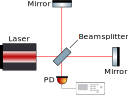
\includegraphics[height=0.5\textwidth,angle=-90]{figures/Michelson_interferometer.pdf}
	\end{center}
	\caption{Configuration of a simple Michelson interferometer}
	\label{fig:Michelson}
\end{figure*}

In its simplest form (ignoring spatial effects henceforth), a Michelson interferometer consists of a laser, a beamsplitter, two arm mirrors, and a photodiode. The laser light is split and travels down two arms, reflects of a mirror at the end of each arm, and then recombines at the beamsplitter output, at which a photodiode is placed. The relative path difference between the two arms produces interference at the photodiode. By tuning the unperturbed lengths of the arms the photodiode can default to being the darkport of the interferometer (or in practise, slightly off the darkport). As such, if something perturbs the arms (e.g.\ noise or a gravitational wave) in a manner to change the relative path difference, then the photodiode will measure some light.


\subsection{Configuration of aLIGO}
% (not investigated here): external squeezing, mode cleaning and spatial effects

\begin{figure*}
	\begin{center}
	\includegraphics[width=0.7\textwidth]{figures/aLIGO_internal_squeezing.pdf}
	\end{center}
	\caption{Simplified configuration of aLIGO}
	\label{fig:aLIGO_configuration}
\end{figure*}

In the farfield, a gravitational wave stretches and squishes the distances between objects in a quadrupole manner. Transverse to the axis of propagation distances in one direction are stretched while those in the perpendicular direction are squished. In order to best detect these changes we need two pairs of objects at right angles to each other (and, ideally, to the gravitational wave). For this we introduce another mirror into each of the beam arms, forming an overcoupled arm cavity between an initial test mass (ITM) and an end test mass (ETM).


% arm cavities, prc, src, 
To achieve the sensitivity required for gravitational wave detection, a classical Michelson interferometer requires technically infeasible amounts of power in the arms. {\Large to-do: Why do we need high power and ITMs???}
To achieve high power in the arms, a power recycling mirror (PRM) is introduced before the beamsplitter, this reflects power returning from the arm cavities back into the interferometer. For reference, in aLIGO a $125$ W laser results in $\approx 5$ kW of power incident on the beam splitter and beyond $600$ kW of power in the arms.


For a passing gravitational wave to result in detectable changes in the arm lengths, the beam arms need to be at least kilometres long (e.g.\ $4$ km long in aLIGO). To increase sensitivity, the signal from the darkport of the beamsplitter can be amplified by reflecting it back into the arms to ``see'' the gravitational wave again. This is done by placing a signal recycling mirror (SRM) after the darkport of the beamsplitter. What the signal recycling cavity (SRC) actually does is more complicated, see Section~\ref{sec:long_srcs}.

\subsubsection{Reduction of aLIGO to coupled cavities}
% simplification to coupled cavities


\subsection{Noise sources}

% strain plot, quantum noise limited strain sensitivity
% quantum, Newtonian (seismic), thermal,


\subsection{Short versus long signal recycling cavities}
\label{sec:long_srcs}

\subsection{Internal squeezing}

% vacuum input, signal and noise see the interferometer differently
% Flucuation Dissipation Theorem~\cite{Danilishin_2012}, loss at an optical component is always accompanied by new un-correlated noise
% quantum noise enters at every open port and every lossy optic


%%%%%%%%%%%%%%%%%%%%%%%%%%%%%%%%%%%%%%%%%%
\section{Modelling a squeezed cavity} %a non-linear element in a cavity
\label{sec:sqzcavity}


\begin{figure*}
	\begin{center}
	\includegraphics[height=0.7\textwidth, angle=-90]{figures/squeezed_cavity.pdf}
	\end{center}
	\caption{Configuration of squeezed cavity}
	\label{fig:squeezed_cavity}
\end{figure*}

\subsection{Analytic derivation}

% perhaps leave the actual derivation to an appendix?
% approximate noise sources to just come from ...

\subsubsection{Threshold}
% threshold results, operating above threshold isn’t physically meaningful for the approximations made to reach these analytics


\subsection{Finesse comparison}



\section{Modelling advanced gravitational wave detector configurations}
\label{sec:aLIGOcomparison}
% \subsection{Analytics for aLIGO}
% \subsection{Finesse simulation for aLIGO}
% \subsection{Comparison for long SRC with internal squeezing}


\subsection{Reasons for the discrepancy}

% different def of dB gives a factor of 2
% double passing of NLE gives another factor of 2
% => gave to input to NLE 1/4 of the input to analytics

% approximations in the analytics
 % (including the calculation of the coupled cavity pole, the interferometer itself!) 

% Is the recommendation to Daniel Brown to both fix the dB and make nle a directional component (will squeeze light from n1 to n2, but will just let light through n2 to n1)?


%%%%%%%%%%%%%%%%%%%%%%%%%%%%%%%%%%%%%%%%%%
\section{Future work}
\label{sec:future_work}

% (detuned long SRC ,non degenerate squeezing, limitations of finesse in its current form that can be overcome)


\section{Conclusions}
\label{sec:conclusions}


\begin{acknowledgments}



\end{acknowledgments}


\appendix
% don’t bother with subfiles just yet
% \subfile{appendix.tex}


\nocite{*}
\bibliographystyle{myunsrt}
\bibliography{bib}


\end{document}
